\section{Описание}

Булев индекс представляет собой инвертированную структуру данных, которая отображает уникальные термины на списки идентификаторов документов (номера документов, в которых встречается термин). \\ \\
Основная задача индекса — обеспечить быстрый поиск документов по терминам с возможностью выполнения булевых операций. В данной работе реализовано построение индекса с использованием алгоритма \textbf{SPIMI (Single-Pass In-Memory Indexing)}, что позволяет эффективно обрабатывать коллекции документов большего объема, чем доступно оперативной памяти.

\vspace{1 em}
\noindent\textbf{Формат хранения инвертированного индекса.} Имеется два уровня представления:
\begin{enumerate}
    \item \textbf{В памяти:} Для временного хранения терминов и их постлистов используется хэш-таблица фиксированного размера с цепочками для разрешения коллизий. Каждый элемент таблицы содержит термин (строка), односвязный список идентификаторов документов и указатель на следующий элемент.
    \item \textbf{На диске:} Финальный индекс сохраняется в бинарном файле с определенной структурой, состоящей из заголовка, словаря терминов и секции постлистов.
\end{enumerate}

\pagebreak

\section{Исходный код}

\vspace{1 em}
\noindent\textbf{Формат хранения инвертированного индекса.} Имеются два уровня представления:
\begin{enumerate}
    \item \textbf{В памяти:} Для временного хранения терминов и их постлистов используется хэш-таблица фиксированного размера с цепочками для разрешения коллизий. Каждый элемент таблицы содержит термин (строка), односвязный список идентификаторов документов и указатель на следующий элемент.
    \item \textbf{На диске:} Финальный индекс сохраняется в бинарном файле с определённой структурой, состоящей из заголовка, словаря терминов и секции постлистов.
\end{enumerate}

\noindent\textbf{Алгоритм построения индекса SPIMI.}

\begin{enumerate}
    \item \textbf{Чтение коллекции документов:} Файлы с расширением .txt в указанной директории сортируются по числовому идентификатору, извлеченному из имени файла.
    \item \textbf{Индексация:} Для каждого документа выполняется чтение токенов. Для каждого уникального в рамках документа токена добавляется запись в индекс: термин ассоциируется с идентификатором текущего документа. Подсчитывается потребление памяти структурой индекса.
    \item \textbf{Запись промежуточного блока (индекса):} При достижении заданного лимита памяти текущее состояние индекса (хэш-таблица) сортируется по терминам в лексикографическом порядке и записывается на диск в виде отдельного блока (файл `block\_X.bin`). Формат блока: количество терминов, затем для каждого термина — длина строки, сам термин, количество документов в постлисте и список идентификаторов документов.
    \item \textbf{Слияние блоков:} После обработки всего корпуса все промежуточные блоки сливаются в единый индекс. На каждом шаге выбирается лексикографически наименьший термин среди текущих терминов всех блоков, объединяются его постлисты из всех блоков (удаляются дубликаты, сохраняется сортировка по возрастанию ID из-за того что обрабатывали документы по очереди), и результат записывается в финальный индекс. Этот процесс повторяется до исчерпания всех терминов во всех блоках.
    \item \textbf{Формирование финального файла:} Финальный индекс записывается в файл `final\_index.bin`. Промежуточные блоки удаляются. \\
    
    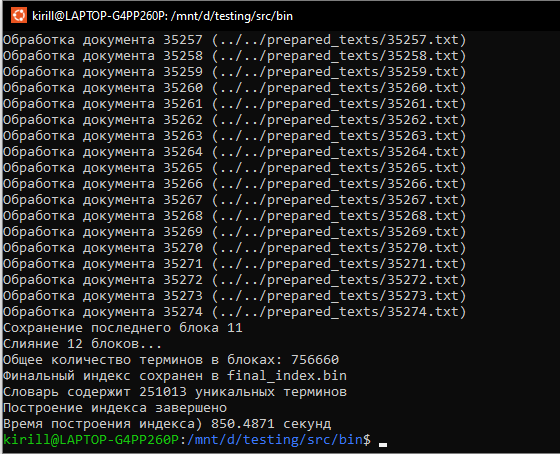
\includegraphics[width=\textwidth, height=\textheight, keepaspectratio]{pics/indexing.png}
\end{enumerate}

\pagebreak

\vspace{1 em}
\noindent\textbf{Структура бинарного файла финального индекса.}

\begin{verbatim}
+-----------------------------------+ <-- Начало файла (offset 0)
|          Заголовок (29 байт)      |
|-----------------------------------|
| Сигнатура (0x42584449)            |  # 4 байта, uint32_t
| Версия формата (1)                |  # 1 байт, uint8_t
| Размер словаря (N)                |  # 8 байт, uint64_t
| Смещение на начало постлистов     |  # 8 байт, uint64_t
| Размер секции постлистов в байтах |  # 8 байт, uint64_t
+-----------------------------------+
|          Словарь терминов         |
|-----------------------------------|
| Термин 1:                         |
|   Длина термина (L1)              |  # 4 байта, uint32_t
|   Символы термина (L1 байт)       |  # сам термин
|   Смещение до постлиста (O1)      |  # 8 байт, uint64_t
|   Количество документов (C1)      |  # 4 байта, uint32_t
|-----------------------------------|
| Термин 2:                         |
|   Длина термина (L2)              |
|   Символы термина (L2 байт)       |
|   Смещение до постлиста (O2)      |
|   Количество документов (C2)      |
| ...                               |
+-----------------------------------+ <-- Смещение postings_start
|         Секция постлистов         |
|-----------------------------------|
| Постлист 1:                       |
|   ID документа 1.1                |  # 4 байта, uint32_t
|   ID документа 1.2                |  # 4 байта
|   ... (всего C1 записей)          |
|-----------------------------------|
| Постлист 2:                       |
|   ID документа 2.1                |  # 4 байта
|   ID документа 2.2                |  # 4 байта
|   ... (всего C2 записей)          |
| ...                               |
+-----------------------------------+ <-- Конец файла
\end{verbatim}

\pagebreak

\noindent\textbf{Сериализация и десериализация индекса.}

\begin{itemize}
    \item \textbf{Сериализация (сохранение).} Финальный индекс формируется в процессе слияния блоков. Заголовок записывается в начале файла, за ним следует словарь, где каждый термин сопровождается метаданными: длина термина, сам термин, смещение относительно начала секции постлистов (не начала файла) и количество документов в постлисте. Постлисты записываются в отдельную секцию, на начало которой указывает поле `postings\_start` в заголовке. \\

\begin{lstlisting}[language=C]
void build_index( const char * input_dir )
{
    printf( "Начало построения индекса...\n" );
    printf( "Входная директория: %s\n", input_dir );
    
    int file_count = 0;
    char ** files = get_sorted_files( input_dir, &file_count );
    if ( file_count == 0 )
    {
        printf( "В директории нет .txt файлов\n" );
        return;
    }
    
    printf( "Найдено %d файлов\n", file_count );
    
    SPIMIIndex * index = create_spimi_index();
    int block_id = 0;
    char ** block_files = NULL;
    int block_count = 0;
    
    for ( int i = 0; i < file_count; i++ )
    {
        uint32_t doc_id = extract_doc_id( files[i] );
        printf( "Обработка документа %u (%s)\n", doc_id, files[i] );
        
        FILE * file = fopen( files[i], "r" );
        if ( !file )
        {
            fprintf( stderr, "Ошибка открытия файла: %s (errno: %d)\n", files[i], errno );
            continue;
        }
        
        char token[MAX_TERM_LEN];
        char unique_tokens[1000][MAX_TERM_LEN];
        int unique_count = 0;
        
        while ( fscanf( file, "%255s", token ) == 1 )
        {
            int is_unique = 1;
            for ( int j = 0; j < unique_count; j++ )
            {
                if ( strcmp( token, unique_tokens[j] ) == 0 )
                {
                    is_unique = 0;
                    break;
                }
            }
            
            if ( is_unique )
            {
                if ( unique_count < 1000 )
                {
                    strcpy( unique_tokens[unique_count], token );
                    add_posting( index, token, doc_id );
                    unique_count++;
                }
            }
        }
        
        fclose( file );
        
        if ( index->mem_usage > MEMORY_LIMIT )
        {
            printf( "Достигнут лимит памяти, сохранение блока %d\n", block_id );
            write_spimi_block( index, block_id );
            
            block_files = realloc( block_files, ( block_count + 1 ) * sizeof( char * ) );
            block_files[block_count] = malloc( 50 );
            sprintf( block_files[block_count], "block_%d.bin", block_id );
            block_count++;
            
            free_spimi_index( index );
            index = create_spimi_index();
            
            block_id++;
        }
    }
    
    if ( index->count > 0 )
    {
        printf( "Сохранение последнего блока %d\n", block_id );
        write_spimi_block( index, block_id );
        
        block_files = realloc( block_files, ( block_count + 1 ) * sizeof( char * ) );
        block_files[block_count] = malloc( 50 );
        sprintf( block_files[block_count], "block_%d.bin", block_id );
        block_count++;
    }
    
    free_spimi_index( index );
    
    for ( int i = 0; i < file_count; i++ )
    {
        free( files[i] );
    }
    free( files );
    
    if ( block_count > 0 )
    {
        printf( "Слияние %d блоков...\n", block_count );
        merge_blocks( block_count );
        
        remove_intermediate_files( block_count );
        
        for ( int i = 0; i < block_count; i++ )
        {
            free( block_files[i] );
        }
        free( block_files );
    }
    
    printf( "Построение индекса завершено\n" );
}
\end{lstlisting}

    
    \item \textbf{Десериализация (загрузка).} При загрузке индексного файла сначала проверяется сигнатура и версия формата. Затем читается словарь. Для ускорения поиска термина при выполнении запросов словарь загружается не только в массив (для последовательного доступа), но и в хэш-таблицу. Хэш-таблица использует простое хэширование с цепочками, что обеспечивает амортизированное время поиска O(1). Каждый элемент хэш-таблицы содержит термин, смещение до его постлиста и количество документов. Сами постлисты остаются на диске и считываются по запросу при помощи функции `get\_postings`, которая перемещается к нужному смещению в файле и читает указанное количество ID документов. \\


\begin{lstlisting}[language=C]
IndexHandle * load_index( const char * file_path )
{
    IndexHandle * handle = malloc( sizeof( IndexHandle ) );
    handle->file_path = strdup( file_path );
    handle->file_handle = NULL;
    handle->dictionary_array = NULL;
    handle->dict_size = 0;
    
    FILE * file = fopen( file_path, "rb" );
    if ( !file )
    {
        perror( "Ошибка открытия индекса" );
        free( handle->file_path );
        free( handle );
        return NULL;
    }
    
    uint32_t magic;
    uint8_t version;
    uint64_t dict_size;
    
    fread( &magic, sizeof( uint32_t ), 1, file );
    fread( &version, sizeof( uint8_t ), 1, file );
    
    if ( magic != MAGIC_NUMBER || version != 1 )
    {
        fprintf( stderr, "Неверный формат файла индекса: magic=%x, version=%d\n", magic, version );
        fclose( file );
        free( handle->file_path );
        free( handle );
        return NULL;
    }
    
    fread( &dict_size, sizeof( uint64_t ), 1, file );
    fread( &handle->postings_start, sizeof( uint64_t ), 1, file );
    
    uint64_t postings_size;
    fread( &postings_size, sizeof( uint64_t ), 1, file );
    
    if ( dict_size > 10000000 )
    {
        fprintf( stderr, "Слишком большое количество терминов: %lu. Файл поврежден?\n", dict_size );
        fclose( file );
        free( handle->file_path );
        free( handle );
        return NULL;
    }
    
    printf( "Загрузка словаря из %lu терминов...\n", dict_size );
    
    uint32_t hash_table_size = ( uint32_t ) ( dict_size * 2 );
    if ( hash_table_size < 1024 ) hash_table_size = 1024;
    handle->hash_table = create_dict_hash_table( hash_table_size );
    
    handle->dictionary_array = malloc( dict_size * sizeof( DictionaryEntry ) );
    handle->dict_size = ( uint32_t ) dict_size;
    
    for ( uint64_t i = 0; i < dict_size; i++ )
    {
        uint32_t term_len;
        if ( fread( &term_len, sizeof( uint32_t ), 1, file ) != 1 )
        {
            fprintf( stderr, "Ошибка чтения длины термина %lu\n", i );
            fclose( file );
            free_dict_hash_table( handle->hash_table );
            free( handle->dictionary_array );
            free( handle->file_path );
            free( handle );
            return NULL;
        }
        
        if ( term_len > MAX_TERM_LEN )
        {
            fprintf( stderr, "Термин %lu слишком длинный: %u (макс: %d)\n", i, term_len, MAX_TERM_LEN );
            fclose( file );
            free_dict_hash_table( handle->hash_table );
            free( handle->dictionary_array );
            free( handle->file_path );
            free( handle );
            return NULL;
        }
        
        char * term = malloc( term_len + 1 );
        if ( fread( term, 1, term_len, file ) != term_len )
        {
            fprintf( stderr, "Ошибка чтения термина %lu\n", i );
            free( term );
            fclose( file );
            free_dict_hash_table( handle->hash_table );
            free( handle->dictionary_array );
            free( handle->file_path );
            free( handle );
            return NULL;
        }
        term[term_len] = '\0';
        
        uint64_t offset;
        uint32_t count;
        
        if ( fread( &offset, sizeof( uint64_t ), 1, file ) != 1 )
        {
            fprintf( stderr, "Ошибка чтения offset для термина %lu\n", i );
            free( term );
            fclose( file );
            free_dict_hash_table( handle->hash_table );
            free( handle->dictionary_array );
            free( handle->file_path );
            free( handle );
            return NULL;
        }
        
        if ( fread( &count, sizeof( uint32_t ), 1, file ) != 1 )
        {
            fprintf( stderr, "Ошибка чтения count для термина %lu\n", i );
            free( term );
            fclose( file );
            free_dict_hash_table( handle->hash_table );
            free( handle->dictionary_array );
            free( handle->file_path );
            free( handle );
            return NULL;
        }
        
        dict_hash_table_insert( handle->hash_table, term, offset, count );
        
        handle->dictionary_array[i].term = term;
        handle->dictionary_array[i].offset = offset;
        handle->dictionary_array[i].count = count;
    }
    
    fclose( file );
    handle->file_handle = NULL;
    
    printf( "Индекс загружен. Хэш-таблица содержит %u терминов\n",
            handle->hash_table->count );
    printf( "Коэффициент заполнения: %.2f\n",
            ( float ) handle->hash_table->count / handle->hash_table->size );
    
    return handle;
}
\end{lstlisting}
\end{itemize}

\pagebreak

